\documentclass[12pt]{article}
\usepackage[english]{babel}
\usepackage{natbib}
\usepackage{url}
\usepackage[utf8x]{inputenc}
\usepackage{amsmath}
\usepackage{graphicx}
\usepackage{subfig}
\graphicspath{{../images/}}
\usepackage{parskip}
\usepackage{fancyhdr}
\usepackage{vmargin}
\usepackage{algorithm}
\usepackage[noend]{algpseudocode}
\newcommand{\var}{\texttt}
\usepackage[toc,page]{appendix}

\setmarginsrb{3 cm}{2.5 cm}{3 cm}{2.5 cm}{1 cm}{1.5 cm}{1 cm}{1.5 cm}

\title{Heuristics \& Approximations Algorithms}								% Title
\author{Alexander \& Narongrit}								% Author
\date{27 May 2019}											% Date

\makeatletter
\let\thetitle\@title
\let\theauthor\@author
\let\thedate\@date
\makeatother

\pagestyle{fancy}
\fancyhf{}
\rhead{\theauthor}
\lhead{\thetitle}
\cfoot{\thepage}

\makeatletter
\let\OldStatex\Statex
\renewcommand{\Statex}[1][3]{%
  \setlength\@tempdima{\algorithmicindent}%
  \OldStatex\hskip\dimexpr#1\@tempdima\relax}
\makeatother

\begin{document}

%%%%%%%%%%%%%%%%%%%%%%%%%%%%%%%%%%%%%%%%%%%%%%%%%%%%%%%%%%%%%%%%%%%%%%%%%%%%%%%%%%%%%%%%%

\begin{titlepage}
	\centering
    \vspace*{0.5 cm}
    
\includegraphics[scale = 0.5]{SDU_logo.png}\\[1.0 cm]	% University Logo
    \textsc{\LARGE University of Southern Denmark}\\[2.0 cm]	% University Name
	\textsc{\Large DM852}\\[0.5 cm]				% Course Code
	\rule{\linewidth}{0.2 mm} \\[0.4 cm]
	{ \huge \bfseries \thetitle}\\
	\rule{\linewidth}{0.2 mm} \\[1.5 cm]
	
	\begin{minipage}{0.4\textwidth}
		\begin{flushleft} \large
			\emph{Submitted To:}\\
			Marco Chiarandini\\
            Lene Monrad Favrholdt \\
			IMADA \\
			Mathematics \& Computer Science Department \\
			\end{flushleft}
			\end{minipage}~
			\begin{minipage}{0.4\textwidth}
            
			\begin{flushright} \large
			\emph{Submitted By :} \\
			Alexander Lerche Falk\\
            Narongrit Unwerawattana\\
            Spring - Master of Computer Science\\
		\end{flushright}
        
	\end{minipage}\\[2 cm]
	
	
    
    
    
    
	
\end{titlepage}

%%%%%%%%%%%%%%%%%%%%%%%%%%%%%%%%%%%%%%%%%%%%%%%%%%%%%%%%%%%%%%%%%%%%%%%%%%%%%%%%%%%%%%%%%

\tableofcontents
\pagebreak

%%%%%%%%%%%%%%%%%%%%%%%%%%%%%%%%%%%%%%%%%%%%%%%%%%%%%%%%%%%%%%%%%%%%%%%%%%%%%%%%%%%%%%%%%

\section{Introduction}

This project shows metaheuristic algorithms, resolving the Capacitated Vehicle Routing Problem (CVRP). The difference between metaheuristics and heuristics is in 
the solution part. For heuristics, you are trying your best to find a solution, even though it is not optimal. The algorithm is adapted to the problem
in such a greedy approach, it can get stuck in a local optimum. This is fine since it is the idea of heuristics: "just solve the problem". 
\newline
Metaheuristics are less greedy and tends to be more problem independent. They accept temporary solutions and allow "bad" steps as an attempt to get
a better solution. You have a local- and global optimum to keep track of the best solution found. You can say metaheuristics are exploting
heuristics to avoid getting trapped. 
\newline
In this metaheuristics implementation project, we have chosen to implement two algorithms for CVRP: Simulated Annealing (SA) and Ant Colony Optimization (ACO). 
The SA algorithm is the one we have uploaded for electronic submisison at http://valkyria.imada.sdu.dk/D0App/. The ACO algorithm is implemented but does not perform well.
We will compare the algorithms with our previous heuristic / local search project and lastly, show our results of computation for our two algorithms.

\hspace{1 cm}--- Alexander \& Narongrit

\newpage

\section{Simulated Annealing} 


The Simulated Annealing (SA) algorithm is inspired from the annealing process in metal, where you are altering the physical state of the metal 
by heating and cooling it. The inspiration can be used in computer science as well. We can use the algorithm on CVRP by starting off by generating a solution 
to the problem and not "care" about the initial solutions. The better steps we are taking, and better solutions we are finding, the more careful we are going to be in finding 
a solution. In the beginning we allow random and bad steps to be performed, while later, we make better calculations.
\newline
In our algorithm we have ... KIE DO SOMETHING HERE
\newline

\begin{algorithm}[!ht]
	\caption{Metaheuristic - Simulated Annealing}\label{euclid}
	\begin{algorithmic}[1]
	
	\end{algorithmic}
\end{algorithm}

\newpage
\section{Ant Colony Optimization}
The Ant Colony Optimization (ACO) algorithm comes from the evolutionary algorithms, where computer science meets nature. In this algorithm, 
we have led us to be inspired by how ants find food in the nature. They are starting by spreading out in some area, randomly. When they seem to find trails, 
which could indicate to be good trails to find food, they leave pheromone behind them. The pheromone is used by other ants to determine their probability of taking 
a trail. If they are standing in a cross-section and they have to choose, they are taking the path with the highest pheromone. 
At some point in their exploration to find the best trail to obtain food, all the ants are using the same trails to get food and get back safe home. 
\newline
We can apply the logic of the ants in the CVRP as well. By letting the instance \- the space of which the requests are "plotted" \- be the area to find a solution, 
we can start by sending one "ant" out to a point. From this point, we are going to calculate every probability of moving to the next point \- the one with the highest "score". 
We can calulate the probabilty of moving by the following: 
\newline
First we establish the initial pheromone levels from all the points to every counter other point: \\

M = \begin{bmatrix}
    0 & 0.50 & 0.20           \\[0.3em]
    0.125 & 0           & 0.60 \\[0.3em]
    1.20 & 0.355 & 0
  \end{bmatrix}

\begin{figure}[H]
	\caption{Illustration of the ACO algorithm, showing how it can be used, and how it process next moves}
	\centering
	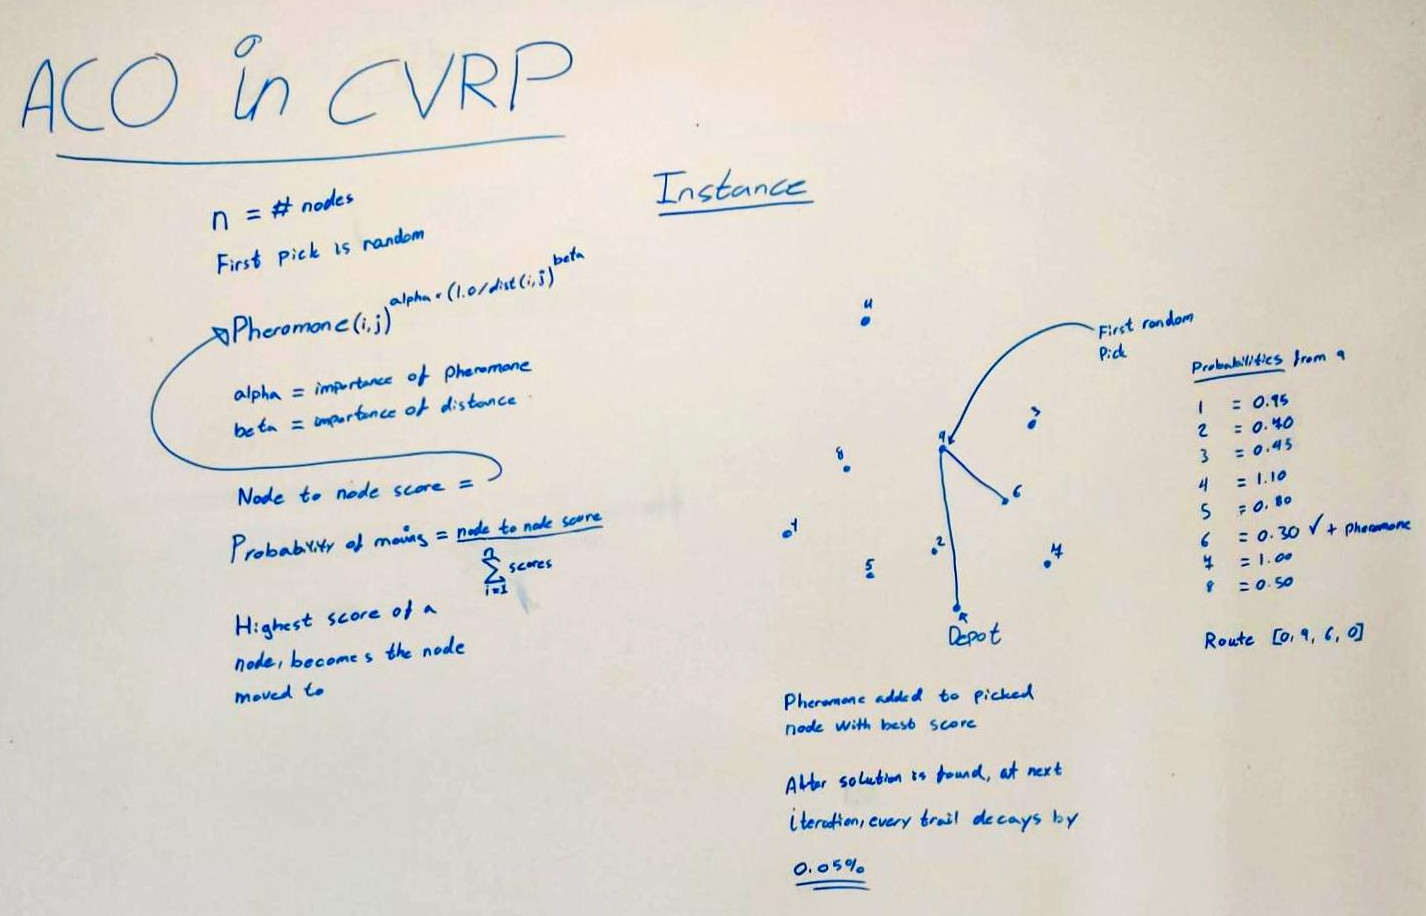
\includegraphics[width=0.9\textwidth]{ACO_Whiteboard.jpg}
	\label{fig:acowhiteboard}

\end{figure}



\section{\\ BOXPLOT FIGURES}

\newpage
\begin{appendices}


\end{appendices}
\end{document}